\documentclass[12pt,letterpaper]{exam}
\usepackage[lmargin=1in,rmargin=1in,tmargin=1in,bmargin=1in]{geometry}
\usepackage{../style/exams}

% -------------------
% Course & Exam Information
% -------------------
\newcommand{\course}{MAT 104: Exam 1}
\newcommand{\term}{Spring -- 2023}
\newcommand{\examdate}{03/03/2023}
\newcommand{\timelimit}{85 Minutes}

\setbool{hideans}{false} % Student: True; Instructor: False

% -------------------
% Content
% -------------------
\begin{document}

\examtitle
\instructions{Write your name on the appropriate line on the exam cover sheet. This exam contains \numpages\ pages (including this cover page) and \numquestions\ questions. Check that you have every page of the exam. Answer the questions in the spaces provided on the question sheets. Be sure to answer every part of each question and show all your work.} 
\scores
%\bottomline
\newpage

% ---------
% Questions
% ---------
\begin{questions}

% Question 1
\newpage
\question[10] Suppose that $f(x)$ is a function with domain $[-10, 10)$ and $g(x)$ is a function with domain $(-5, 15]$. Several outputs for the functions $f(x)$ and $g(x)$ are given below. \par
	\begin{table}[!ht]
	\centering
	\begin{tabular}{|c||c|c|c|c|c|} \hline
	$x$ & $0$ & $1$ & $2$ & $3$ & $5$ \\ \hline \hline
	$f(x)$ & $3$ & $0$ & $2$ & $4$ & $4$ \\ \hline
	$g(x)$ & $3$ & $5$ & $1$ & $2$ & $0$ \\ \hline
	\end{tabular}
	\end{table} \par

\begin{enumerate}[(a)]
\item What is the domain of $f - g$?
\item Given the information above, what is the largest possible domain for $\frac{f}{g}$?
\item Find $(f + g)(2)$.
\item Find $(fg)(0)$.
\item Find $(g \circ f)(0)$.
\end{enumerate} \pspace

{\itshape
\begin{enumerate}[(a)]
\item For $f - g$ to be defined, both $f, g$ need to be defined because $(f - g)(x)= f(x) - g(x)$, so $f(x)$ and $g(x)$ need to be defined. Therefore, the domain of $f - g$ is the `overlap' of the domains for $f(x)$ and $g(x)$. Therefore, the domain of $f - g$ is $(-5, 10)$. 
	\[
	\text{Domain } f - g \colon (-5, 10)
	\]

\item For $\frac{f}{g}$ to be defined, both $f, g$ need to be defined because $\left( \frac{f}{g} \right)(x)= \frac{f(x)}{g(x)}$, so $f(x)$ and $g(x)$ need to be defined. Therefore, the domain of $f - g$ is the `overlap' of the domains for $f(x)$ and $g(x)$. The overlap of these domains is $(-5, 10)$. However, for $\frac{f(x)}{g(x)}$ to be defined, we also need $g(x) \neq 0$. From the table, we see that if $x= 5$, then $g(x)= g(5)= 0$. Therefore, this also cannot be in the domain of $\frac{f}{g}$. Excluding this value from the interval $(-5, 10)$ yields $(-5, 5) \cup (5, 10)$. Therefore, the largest the domain of $\frac{f}{g}$ can be is $(-5, 5) \cup (5, 10)$. 
	\[
	\text{Domain } \dfrac{f}{g} \colon (-5, 5) \cup (5, 10)
	\]

\item We have\dots
	\[
	(f + g)(2)= f(2) + g(2)= 2 + 1= 3
	\] \pspace

\item We have\dots
	\[
	(fg)(0)= f(0) g(0)= 3 \cdot 3= 9 
	\] \pspace 

\item We have\dots
	\[
	(g \circ f)(0)= g\big( f(0) \big)= g(3)= 2 
	\] 
\end{enumerate}
}



% Question 2
\newpage
\question[10] Let $f(x)$ be an exponential function with $f(-2)= 12$ and $f(3)= \frac{3}{8}$. Showing all your work, find $f(x)$. \pspace

{\itshape
\sol Because $f(x)$ is an exponential function, we know that $f(x)= ab^x$ for some $a, b$. But then we know\dots
	\[
	\begin{aligned}
	f(-2)&= ab^{-2} \\
	f(3)&= ab^3
	\end{aligned}
	\]
But using the fact that $f(-2)= 12$ and $f(3)= \frac{3}{8}$, we know\dots
	\[
	\begin{aligned}
	12&= ab^{-2} \\
	\frac{3}{8}&= ab^3
	\end{aligned}
	\]
Dividing each of these, we have\dots
	\[
	\dfrac{12}{3/8}= \dfrac{a b^{-2}}{a b^3}= \dfrac{\cancel{a} b^{-2}}{\cancel{a} b^3}= \dfrac{b^{-2}}{b^3}= \dfrac{1}{b^5}
	\]
Then using the fact that $\frac{12}{3/8}= 12 \cdot \frac{8}{3}= 4 \cdot 8= 32$. Therefore, we have\dots
	\[
	\begin{aligned}
	\dfrac{1}{b^5}&= 32 \\
	b^5&= \dfrac{1}{32} \\
	b&= \sqrt[5]{\dfrac{1}{32}} \\
	b&= \dfrac{1}{2}
	\end{aligned}
	\]
But then using the fact that $12= ab^{-2}$, we have\dots
	\[
	12= ab^{-2}= a \left( \dfrac{1}{2} \right)^{-2}= a \cdot 2^2= 4a
	\]
But then $a= \frac{12}{4}= 3$. Therefore, we know that\dots
	\[
	f(x)= 3 \left( \dfrac{1}{2} \right)^x
	\]
}



% Question 3
\newpage
\question[10] Showing all your work, find the inverse of the function $f(x)= \log_3(x^2) - 4$. \pspace

{\itshape
\sol We have\dots
	\[
	\begin{gathered}
	f(x)= \log_3(x^2) - 4 \\[0.3cm]
	y= \log_3(x^2) - 4 \\[0.3cm]
	\Downarrow \\[0.3cm]
	x= \log_3(y^2) - 4 \\[0.3cm]
	x= 2 \log_3(y) - 4 \\[0.3cm]
	x + 4= 2 \log_3(y) \\[0.3cm]
	\dfrac{x + 4}{2}= \log_3(y) \\[0.3cm]
	3^{\frac{x + 4}{2}}= 3^{\log_3(y)} \\[0.3cm]
	y= 3^{\frac{x + 4}{2}} \\[0.3cm]
	f^{-1}(x)= 3^{\frac{x + 4}{2}}
	\end{gathered}
	\] \pspace
We can also verify that this is the inverse:
	\[
	\begin{aligned}
	(f \circ f^{-1}(x)= f \big( f^{-1}(x) \big)= f \left( 3^{\frac{x + 4}{2}} \right)= \log_3 \left( \left( 3^{\frac{x + 4}{2}} \right)^2 \right) - 4= \log_3 \left( 3^{x + 4} \right) - 4= (x + 4) - 4= x \\[0.3cm]
	(f^{-1} \circ f)(x)= f^{-1} \big( f(x) \big)= f^{-1} \left( \log_3(x^2) - 4 \right)= 3^{\frac{\log_3(x^2) - 4 + 4}{2}}= 3^{\frac{\log_3(x^2)}{2}}= 3^{\frac{2\log_3(x)}{2}}= 3^{\log_3(x)}= x
	\end{aligned}
	\]
}



% Question 4
\newpage
\question[10] A function $f(x)$ is plotted below. As accurately as possible, sketch the function $4 - f(x + 3)$ on the graph below. 
	\[
	\fbox{
	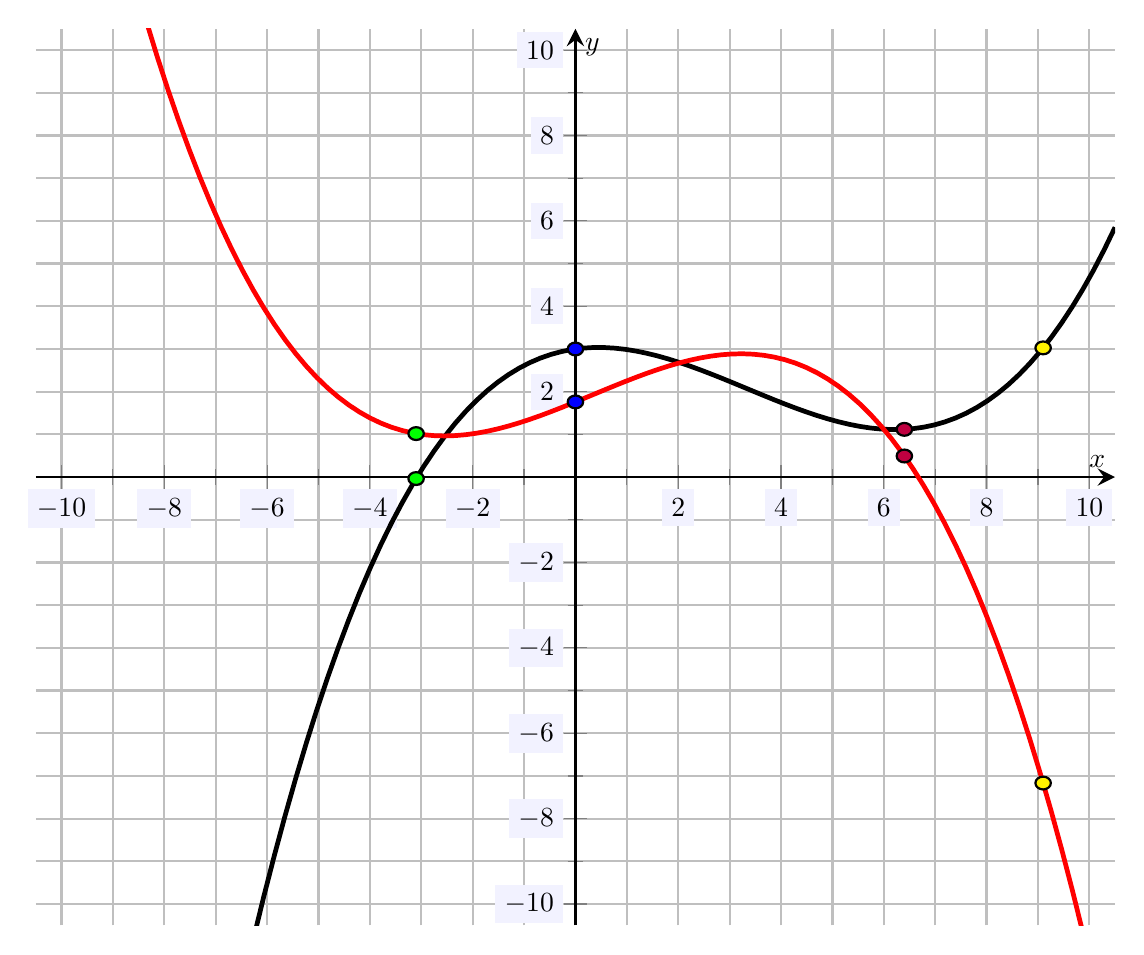
\begin{tikzpicture}[scale=2,every node/.style={scale=0.5}]
	\begin{axis}[
	grid=both,
	axis lines=middle,
	ticklabel style={fill=blue!5!white},
	xmin= -10.5, xmax=10.5,
	ymin= -10.5, ymax=10.5,
	xtick={-10,-8,...,10},
	ytick={-10,-8,...,10},
	minor x tick num = 1,
	minor y tick num = 1,
	xlabel=\(x\),ylabel=\(y\),
	]
	\addplot[domain=-10:10.5,samples=100,line width=0.03cm] (x,1/50*x^3 - 1/5*x^2 + 1/6*x + 3);
	\addplot[red,domain=-10:10.5,samples=100,line width=0.03cm] (x,44/25 + 37/75*x + x^2/50 - x^3/50);
	\draw[fill=yellow] (9.1,3.02609) circle (0.15);
	\draw[fill=blue] (0,3) circle (0.15);
	\draw[fill=green] (-3.1,-0.0344867) circle (0.15);
	\draw[fill=purple] (6.4,1.11755) circle (0.15);
	
	\draw[fill=yellow] (9.1,-7.16589) circle (0.15);
	\draw[fill=blue] (0,44/25) circle (0.15);
	\draw[fill=green] (-3.1,1.01869) circle (0.15);
	\draw[fill=purple] (6.4,0.493653) circle (0.15);
	\end{axis}
	\end{tikzpicture}
	}
	\] \pspace

{\itshape
\sol Compared to $f(x)$, the graph of $f(x + 3)$ is shifted 3 to the left. Compared to the graph of $f(x)$, the graph of $-f(x + 3)$ is shifted 3 to the left and then reflected across the $x$-axis. Finally, compared to the graph of $f(x)$, the graph of $f(x)$, the graph of $4 - f(x + 3)$ is shifted 3 to the left, reflected across the $x$-axis, and shifted up by 4. We can then sketch the function $4 - f(x + 3)$ above. We can also transform several points on the original graph as described above to find the resulting point and connect these to sketch the graph $4 - f(x + 3)$. These are shown by matching colored points on the plot above. 
}



% Question 5
\newpage
\question[10] Let $f(x)= 3 - 2x$ and $g(x)= x^2 + x - 1$. Showing all your work and simplifying as much as possible, find the following:
	\begin{enumerate}[(a)]
	\item $f \big( g(0) \big)$
	\item $(2f - g)(0)$
	\item $(g - f)(x)$
	\item $(f \circ g)(x)$
	\item $(g \circ f)(x)$
	\end{enumerate} \pspace

{\itshape
\sol 
\begin{enumerate}[(a)]
\item We have\dots
	\[
	f \big( g(0) \big)= f(0^2 + 0 - 1)= f(0 + 0 - 1)= f(-1)= 3 - 2(-1)= 3 + 2= 5
	\] \pspace

\item We have\dots
	\[
	\hspace{-1.5cm} (2f - g)(0)= 2f(0) - g(0)= 2 \big(3 - 2(0) \big) - (0^2 + 0 - 1)= 2 (3 - 0) - (0 + 0 - 1)= 2(3) - (-1)= 6 + 1= 7
	\] \pspace
 
\item We have\dots
	\[
	\hspace{-0.75cm} (g - f)(x)= g(x) - f(x)= (x^2 + x - 1) - (3 - 2x)= x^2 + x - 1 - 3 + 2x= x^2 + 3x - 4= (x - 1)(x + 4)
	\] \pspace
 
\item We have\dots
	\[
	(f\, \circ\, g)(x)= f \big( g(x) \big)= f(x^2 + x - 1)= 3 - 2(x^2 + x - 1)= 3 - 2x^2 - 2x + 2= -2x^2 - 2x + 5
	\] \pspace
 
\item We have\dots
	\[
	\hspace{-1.5cm} (g\, \circ\, f)(x)= g \big( f(x) \big)= g(3 - 2x)= (3 - 2x)^2 + (3 - 2x) - 1= (4x^2 - 12x + 9) + (3 - 2x) - 1= 4x^2 - 14x + 11
	\]  
\end{enumerate}
}



% Question 6
\newpage
\question[10] Showing all your work, find the inverse of the function $f(x)= 3e^{1 - 2x}$. \pspace

{\itshape 
\sol We have\dots
	\[
	\begin{gathered}
	f(x)= 3e^{1 - 2x} \\[0.3cm]
	y= 3e^{1 - 2x} \\[0.3cm]
	\Downarrow \\[0.3cm]
	x= 3e^{1 - 2y} \\[0.3cm]
	\dfrac{x}{3}= e^{1 - 2y} \\[0.3cm]
	\ln\left( \dfrac{x}{3} \right)= \ln \left( e^{1 - 2y} \right) \\[0.3cm]
	\ln\left( \dfrac{x}{3} \right)= 1 - 2y \\[0.3cm]
	2y= 1 - \ln\left( \dfrac{x}{3} \right) \\[0.3cm]
	y= \dfrac{1 - \ln\left( \dfrac{x}{3} \right)}{2} \\[0.3cm]
	f^{-1}(x)= \dfrac{1 - \ln\left( \dfrac{x}{3} \right)}{2}
	\end{gathered}
	\] \pspace
We can also verify that this is the inverse:
	\[
	\begin{aligned}
	\hspace{-3.1cm} (f \circ f^{-1}(x)&= f \big( f^{-1}(x) \big)= f \left( \frac{1 - \ln\left( \frac{x}{3} \right)}{2} \right)= 3 e^{1 - 2 \cdot \frac{1 - \ln\left( \frac{x}{3} \right)}{2}}= 3e^{1 - (1 - \ln\left( \frac{x}{3} \right)}= 3e^{1 - 1 + \ln\left( \frac{x}{3} \right)}= 3e^{\ln\left( \frac{x}{3} \right)}= 3 \cdot \dfrac{x}{3}= x \\[0.3cm]
	\hspace{-3.1cm} (f^{-1} \circ f)(x)&= f^{-1} \big( f(x) \big)= f^{-1} \left( 3e^{1 - 2x} \right)= \dfrac{1 - \ln\left( \dfrac{3e^{1 - 2x}}{3} \right)}{2}= \dfrac{1 - \ln \left( e^{1 - 2x} \right)}{2}= \dfrac{1 - (1 - 2x)}{2}= \dfrac{1 - 1 + 2x}{2}= \dfrac{2x}{2}= x
	\end{aligned}
	\]
}



% Question 7
\newpage
\question[10] Let $f(x)$ be the function $f(x)= \dfrac{2^{3x + 1}}{5^{1 - x}}$.
	\begin{enumerate}[(a)]
	\item Write $f(x)$ in the form $ab^x$ for some $a$, $b$. 
	\item Is $f(x)$ increasing or decreasing?
	\item Is $f(x)$ concave up or concave down?
	\end{enumerate} \pspace

{\itshape
\sol 
\begin{enumerate}[(a)]
\item We have\dots
	\[
	f(x)= \dfrac{2^{3x + 1}}{5^{1 - x}}= \dfrac{2^{3x} \cdot 2}{5 \cdot 5^{-x}}= \dfrac{2}{5} \cdot \dfrac{2^{3x}}{5^{-x}}= \dfrac{2}{5}  \left( (2^3)^x \cdot 5^x \right)= \dfrac{2}{5} \left( 8^x \cdot 5^x \right)= \dfrac{2}{5} \left(8 \cdot 5 \right)^x= \dfrac{2}{5}\, \cdot\, 40^x
	\]
Therefore, $f(x)$ has the form $ab^x$ with $a= \frac{2}{5}$ and $b= 40$. \pspace

\item Because $f(x)= \frac{2}{5} \cdot 40^x$ has the form $ab^x$ with $a= \frac{2}{5}$ and $b= 40$, because $b= 40 > 1$ and $a= \frac{2}{5} > 0$, the function $f(x)$ is increasing. \pspace

\item Because $f(x)= \frac{2}{5} \cdot 40^x$ has the form $ab^x$ with $a= \frac{2}{5}$ and $b= 40$, because $b= 40 > 1$ and $a= \frac{2}{5} > 0$, the function $f(x)$ is concave up.  
\end{enumerate}
}



% Question 8
\newpage
\question[10] Showing all your work, find the exact solution to the following:
	\[
	\log_2 \left( 50 - e^{x + 1} \right) + 5= 10
	\] \pspace

{\itshape
\sol 
	\[
	\begin{gathered}
	\log_2 \left( 50 - e^{x + 1} \right) + 5= 10 \\[0.3cm]
	\log_2 \left( 50 - e^{x + 1} \right)= 5 \\[0.3cm]
	2^{\log_2 \left( 50 - e^{x + 1} \right)}= 2^5 \\[0.3cm]
	50 - e^{x + 1}= 32 \\[0.3cm]
	e^{x + 1}= 18 \\[0.3cm]
	\ln \left( e^{x + 1} \right)= \ln 18 \\[0.3cm]
	x + 1= \ln 18 \\[0.3cm]
	x= \ln(18) - 1
	\end{gathered}
	\] \pspace
We can also verify this solution: 
	\[
	\begin{gathered}
	\log_2 \left( 50 - e^{x + 1} \right) + 5= 10 \\[0.3cm]
	\log_2 \left( 50 - e^{\ln(18) - 1 + 1} \right) + 5\stackrel{?}{=}10 \\[0.3cm]
	\log_2 \left( 50 - e^{\ln(18)} \right) + 5\stackrel{?}{=}10 \\[0.3cm]
	\log_2 \left( 50 - 18 \right) + 5\stackrel{?}{=}10 \\[0.3cm]
	\log_2(32) + 5 \stackrel{?}{=}10 \\[0.3cm]
	5 + 5\stackrel{?}{=}10 \\[0.3cm]
	10= 10 \\
	\text{\cmark}
	\end{gathered}
	\]
}



% Question 9
\newpage
\question[10] Showing all your work, write the following as a sum of terms involving only $\log_2(x)$, $\log_2(y)$, and possibly a constant:
	\[
	\log_2 \left( \dfrac{16 \sqrt[3]{x}}{y^{-5}} \right)
	\] \pspace

{\itshape
\sol 
	\[
	\begin{aligned}
	\log_2 \left( \dfrac{16 \sqrt[3]{x}}{y^{-5}} \right)&= \log_2 \left( 16 \sqrt[3]{x} \right) - \log_2(y^{-5}) \\[0.3cm]
	&= \log_2(16) + \log_2(\sqrt[3]{x}) - (-5) \log_2(y) \\[0.3cm]
	&= 4 + \log_2(x^{1/3}) + \log_2(y) \\[0.3cm]
	&= 4 + \frac{1}{3} \log_2(x) + \log_2(y)
	\end{aligned}
	\]
}



% Question 10
\newpage
\question[10] Let $f(x)= 2 - e^x$ and $g(x)= 6 \log_5( 2 - x)$.
	\begin{enumerate}[(a)]
	\item What is the domain of $f(x)$?
	\item What is the range of $f(x)$?
	\item What is the domain of $g(x)$?
	\item What is the range of $g(x)$?
	\end{enumerate} \pspace

{\itshape
\sol 
\begin{enumerate}[(a)]
\item The domain of $f(x)= 2 - e^x$ is the set of all real numbers, $\mathbb{R}= (-\infty, \infty)$. \pspace

\item Because the range of $e^x$ is $(0, \infty)$, the range of $-e^x$ is $(-\infty, 0)$. But then the range of $f(x)= 2 - e^x$ is $(-\infty, 2)$. \pspace

\item For a logarithm to be defined, the input need be positive. But then we need $2 - x > 0$. But then the domain of $g(x)= 6 \log_5(2 - x)$ is $2 > x$, i.e. $x < 2$. Equivalently, the domain of $g(x)$ is $(-\infty, 2)$. \pspace

\item The range of $g(x)= 6 \log_5(2 - x)$ is all real numbers, i.e. $\mathbb{R}= (-\infty, \infty)$. 
\end{enumerate}
}



% Question 11
\newpage
\question[10] Showing all your work, find the exact solution to the following:
	\[
	3^{2x}= 5 \cdot 2^x
	\] 

{\itshape
\sol 
	\[
	\begin{gathered}
	3^{2x}= 5 \cdot 2^x \\[0.3cm]
	\dfrac{3^{2x}}{2^x}= 5 \\[0.3cm]
	\left( \dfrac{3^2}{2} \right)^x= 5 \\[0.3cm]
	\left( \dfrac{9}{2} \right)^x= 5 \\[0.3cm]
	\log_{9/2} \left( \dfrac{9}{2} \right)^x= \log_{9/2}(5) \\[0.3cm]
	x= \log_{9/2}(5) 
	\end{gathered}
	\] \pspace
We can verify the solution:
	\[
	\begin{gathered}
	3^{2x}= 5 \cdot 2^x \\[0.1cm]
	3^{2 \log_{9/2}(5)}\stackrel{?}{=} 5 \cdot 2^{\log_{9/2}(5)} \\[0.1cm]
	3^{\log_{9/2}(5^2)}\stackrel{?}{=} 5 \cdot 2^{\log_{9/2}(5)} \\[0.1cm]
	3^{\log_{9/2}(25)}\stackrel{?}{=} 5 \cdot 2^{\log_{9/2}(5)} \\[0.1cm]
	3^{\ln(25)/\ln(9/2)}\stackrel{?}{=} 5 \cdot 2^{\ln(5)/\ln(9/2)} \\[0.1cm]
	\left( 3^{\ln(25)/\ln(9/2)} \right)^{\ln(9/2)} \stackrel{?}{=} \left( 5 \cdot 2^{\ln(5)/\ln(9/2)} \right)^{\ln(9/2)} \\[0.1cm]
	3^{\ln(25)} \stackrel{?}{=} 5^{\ln(9/2)} \cdot 2^{\ln 5} \\[0.1cm]
	3^{2\ln(5)} \stackrel{?}{=} 5^{\ln(9/2)} \cdot 2^{\ln 5} \\[0.1cm]
	\left( 3^{2\ln(5)} \right)^{1/\ln(5)} \stackrel{?}{=} \left( 5^{\ln(9/2)} \cdot 2^{\ln 5} \right)^{1/\ln(5)} \\[0.1cm]
	3^2 \stackrel{?}{=} 5^{\ln(9/2)/\ln(5)} \cdot 2 \\[0.1cm]
	9 \stackrel{?}{=} 5^{\log_5(9/2)} \cdot 2 \\[0.1cm]
	9 \stackrel{?}{=} \dfrac{9}{2} \cdot 2 \\[0.1cm]
	9= 9 \\
	\text{\cmark}
	\end{gathered}
	\]
}



% Question 12
\newpage
\question[10] A relation $f(x)$ is plotted below.
	\[
	\fbox{
	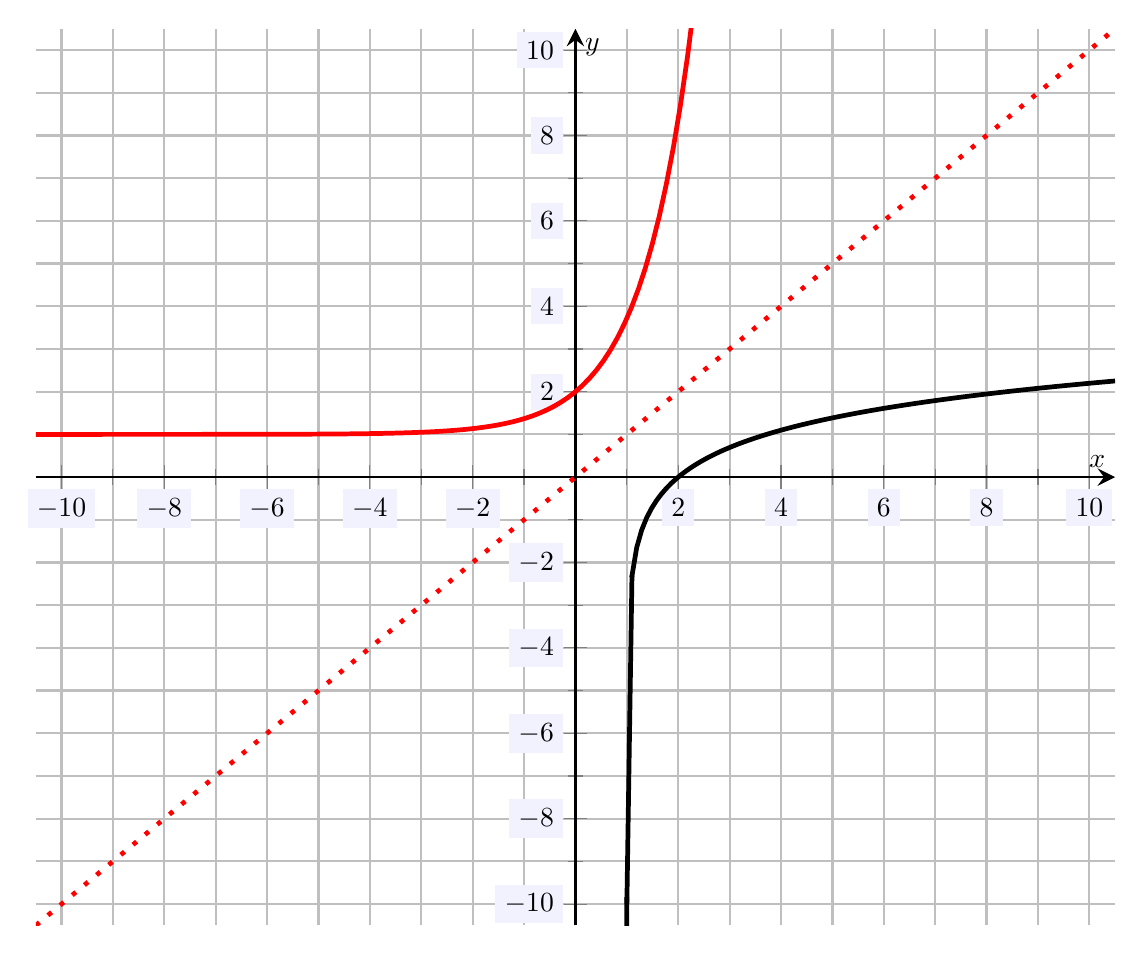
\begin{tikzpicture}[scale=2,every node/.style={scale=0.5}]
	\begin{axis}[
	grid=both,
	axis lines=middle,
	ticklabel style={fill=blue!5!white},
	xmin= -10.5, xmax=10.5,
	ymin= -10.5, ymax=10.5,
	xtick={-10,-8,...,10},
	ytick={-10,-8,...,10},
	minor x tick num = 1,
	minor y tick num = 1,
	xlabel=\(x\),ylabel=\(y\),
	]
	\addplot[domain=1:10.5,samples=100,line width=0.03cm] {ln(x - 1)};
	\addplot[domain=1:1.00005,samples=100,line width=0.03cm] {ln(x - 1)};
	\draw[line width=0.03cm] (1.0006,-10) -- (1.1,-2.3);
	
	\addplot[domain=-10.5:10.5,samples=2,line width=0.03cm,red,dotted] {x};
	
	\addplot[domain=-10.5:3,samples=100,line width=0.03cm,red] {2.718281828^x + 1};
	\end{axis}
	\end{tikzpicture}
	}
	\] 
\begin{enumerate}[(a)]
\item Using the plot above, explain why $f(x)$ is a function.
\item Using the plot above, explain why $f^{-1}(x)$ exists.
\item Sketch the function $f^{-1}(x)$ on the plot above. 
\end{enumerate} \pspace

{\itshape
\sol
\begin{enumerate}[(a)]
\item The relation $f(x)$ passes the vertical line test. Therefore, $f(x)$ is a function. \pspace

\item The function $f(x)$ passes the horizontal line tests. Therefore, $f(x)$ is one-to-one and hence has an inverse, i.e. $f^{-1}(x)$ exists. \pspace

\item To sketch $f^{-1}(x)$, we reflect the function $f(x)$ across the line $y= x$ (the dotted red line above). This gives the inverse function $f^{-1}(x)$, which is plotted as a solid red curve above. 
\end{enumerate}
}



% Question 13
\newpage
\question[10] Showing all your work, write each of the following as a single logarithm involving no negative powers:
	\begin{enumerate}[(a)]
	\item $\ln(x) + 3 \ln(y)$
	\item $\log_5(x) - \log_5(y^{-2})$
	\item $4\log_3(x) - \frac{1}{2} \log_3(y) + 2$
	\end{enumerate} \pspace

{\itshape
\sol 
\begin{enumerate}[(a)]
\item 
	\[
	\ln(x) + 3 \ln(y)= \ln(x) + \ln(y^3)= \ln(xy^3)
	\] \pspace

\item 
	\[
	\log_5(x) - \log_5(y^{-2})= \log_5 \left( \dfrac{x}{y^{-2}} \right)= \log_5(x y^2)
	\] \pspace

\item 
	\[
	\begin{aligned}
	4\log_3(x) - \frac{1}{2} \log_3(y) + 2&= 4\log_3(x) - \frac{1}{2} \log_3(y) + \log_3(3^2) \\[0.3cm]
	&= \log_3(x^4) + \log_3(y^{-1/2}) + \log_3(9) \\[0.3cm]
	&= \log_3(x^4) + \log_3 \left( \dfrac{1}{\sqrt{y}} \right) + \log_3(9) \\[0.3cm]
	&= \log_3 \left( \dfrac{9x^4}{\sqrt{y}} \right)
	\end{aligned}
	\]
\end{enumerate}
}


% Question 14
\newpage
\question[10] Showing all your work, compute the following ``by hand'': 
	\begin{enumerate}[(a)]
	\item $\ln(e^{3/2})$
	\item $\log_5(\sqrt{5})$
	\item $\log_4 \left( \frac{1}{64} \right)$
	\item $\log_9(3)$
	\item $\log_8(128)$
	\end{enumerate} \pspace

{\itshape
\sol 
\begin{enumerate}[(a)]
\item 
	\[
	\ln(e^{3/2})= \dfrac{3}{2}
	\] \pspace 

\item 
	\[
	\log_5(\sqrt{5})= \log_5(5^{1/2})= \dfrac{1}{2}
	\] \pspace 
 
\item 
	\[
	\log_4 \left( \dfrac{1}{64} \right)= \log_4 \left( 64^{-1} \right)= \log_4 \left( (4^3)^{-1} \right)= \log_4 \left( 4^{-3} \right)= -3
	\] \pspace 
 
\item 
	\[
	\log_9(3)= \log_9 (\sqrt{9})= \log_9 (9^{1/2})= \dfrac{1}{2}
	\] \pspace 
 
\item 
	\[
	\log_8(128)= \dfrac{\log_2(128)}{\log_2(8)}= \dfrac{\log_2(2^7)}{\log_2(2^3)}= \dfrac{7}{3}
	\]  
\end{enumerate}
}



% Question 15
\newpage
\question[10] If one invests $P$ dollars at an annual interest rate $r$ (written as a decimal), compounded monthly, then the amount of money in the account after $t$ years, $M(t)$, is given by\dots
	\[
	M(t)= P \left(1 + \dfrac{r}{12} \right)^{12t}
	\]
Suppose that you invest \$8,000 at an annual interest rate of 6.2\%, compounded monthly. 

\begin{enumerate}[(a)]
\item Find the value of the investment after 5~years.
\item Find how long until the investment is worth \$20,000. 
\end{enumerate} \pspace

{\itshape
\sol We have $P= \$8000$ and $r= 0.062$. But then we have\dots
	\[
	M(t)=  P \left(1 + \dfrac{r}{12} \right)^{12t}=  \$8000 \left(1 + \dfrac{0.062}{12} \right)^{12t}=  \$8000 (1.005166667)^{12t}
	\]

\begin{enumerate}[(a)]
\item We have\dots
	\[
	M(5)=  \$8000 (1.005166667)^{12(5)}=  \$8000 (1.005166667)^{60}= \$8000 (1.36233745)= \$10,\!898.70
	\] \pspace

\item We have\dots
	\[
	\begin{gathered}
	M(t)= \$8000 (1.005166667)^{12t} \\[0.3cm]
	\$20000= \$8000 (1.005166667)^{12t} \\[0.3cm]
	(1.005166667)^{12t}= \dfrac{\$20000}{\$8000} \\[0.3cm]
	(1.005166667)^{12t}= 2.5 \\[0.3cm]
	\ln \left( (1.005166667)^{12t} \right)= \ln(2.5) \\[0.3cm]
	12t \ln(1.005166667)= \ln(2.5) \\[0.3cm]
	t= \dfrac{\ln(2.5)}{12 \ln(1.005166667)} \\[0.3cm]
	t \approx \dfrac{0.916291}{0.0618404} \\[0.3cm]
	t \approx 14.817
	\end{gathered}
	\]
\end{enumerate}
}


\end{questions}
\end{document}